\chapter{Vorlesung 6}

\section{Quicksort}

\subsection{Pseudo-Code}
\lstinputlisting[language=C]{6/Code/quicksort.c}

\subsubsection*{}
\begin{wrapfigure}[3]{l}{0.4\linewidth}
\vspace{-40pt}
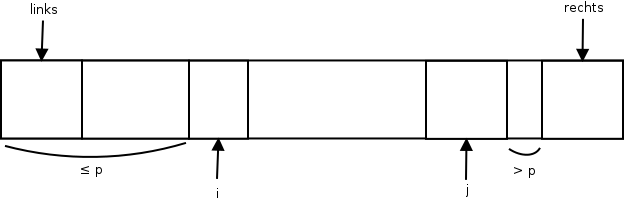
\includegraphics[width=\linewidth]{6/Grafik/img1.png}
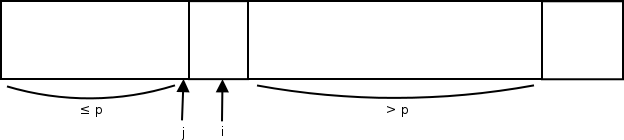
\includegraphics[width=\linewidth]{6/Grafik/img2.png}
\caption{}
\end{wrapfigure}

\vspace{30pt}
\textbf{Schleifen-Invariante:}\\
$a[k] > p~~\text{für}~~j <k<rechts$\\
$a[k] \leq p ~~\text{für}~~links<k<i$ 
\vspace{50pt}

\pagebreak 

\subsection{Zufallspermutation}
\lstinputlisting[language=C]{6/Code/zufallspermutation.c}

\subsection{Einschub: Stochastik}

\subsection{Laufzeitanalyse}


\section{Median in Linearzeit}